\section{Experiments}\label{sec:experiments}
In this section, we describe the experiments conducted to evaluate the performance of the symbolic implementation of the Baum-Welch algorithm in the CuPAAL library by comparing it to the recursive implementation in Jajapy. The evaluation is based on two key aspects: execution time and accuracy.

We conduct two experiments:
\begin{itemize}
    \item \textbf{Performance Comparison} - Measuring runtime and accuracy across different models.
    \item \textbf{Scalability Analysis} - Evaluating performance as the number of states increases.
\end{itemize}

These experiments aim to answer the following research questions:
\begin{itemize}
    \item \textbf{Question 1}: How does the symbolic implementation of the Baum-Welch algorithm in CuPAAL compare to the recursive implementation in Jajapy in terms of runtime and accuracy?
    \item \textbf{Question 2}: How does the performance of the CuPAAL implementation scale with the number of states in the model?
\end{itemize}

\subsection{Experimental Setup}
All experiments are conducted using a set of \glspl{dtmc} and \glspl{ctmc} obtained from publicly available benchmarks\footnote{The models are available at \url{https://qcomp.org/benchmarks/}. The source files describe the parameters and what is observable.}.

Each experiment is run ten times, and results are reported as the average runtime for the full run, average runtime for each iteration,
the average number of iterations, log-likelihood for each iteration, and average relative parameter error for each iteration.
We stop the experiments when we reach a convergence threshold of 0.05, which was the default value in the Jajapy implementation or after
4 hours of runtime.
The training data is randomly generated based on these models, consisting of 30 observation sequences of length 10 for each model.

\subsubsection{Experiment 1: Performance Comparison of Forward-Backward Implementations}
The first experiment is based on the ideas from the experiment conducted in~\cite{reynouard2024learning}.
The models used in this experiment are shown in \autoref{tab:dtmc_models} and \autoref{tab:ctmc_models}.
All models has a fixed number of parameters of, and the number of states varies.

The experiment evaluates the efficiency and accuracy of the symbolic approach (CuPAAL) versus the recursive approach (Jajapy). We measure:
\begin{itemize}
    \item \textbf{Runtime Efficiency} - The average time per run.
    \item \textbf{Convergence Speed} - The average number of iterations required.
    \item \textbf{Accuracy} - Measured using log-likelihood and average relative parameter error.
\end{itemize}

The \textbf{relative parameter error} is calculated as follows $\cfrac{|r-e|}{e}$, where $r$ is the real value and $e$ is the expected value.

\textbf{Log-likelihood:} Measures how well the learned model explains the observed data. Given an observation sequence $O$ and a model $M$, the log-likelihood is calculated as:

$\log P(O \mid M) = \sum_{t=1}^{T} \log P(O_t \mid M)$ where $P(O_t|M)$ is the probability of observing $O_t$ given the model.

Following the approach in \cite{bacci2023mm}, initial parameters are randomly sampled from the range
    [0.00025, 0.0025]. The implementations used are:
\begin{enumerate}
    \item The original Jajapy implementation.
    \item The symbolic CuPAAL implementation.
\end{enumerate}

We expect the CuPAAL implementation to have the same accuracy as the Jajapy implementation and have the same number of iterations. However, we expect the CuPAAL implementation to be faster due to the symbolic approach, which can avoid redundant calculations.

The results are presented for \glspl{dtmc} in \autoref{tab:leader_results}, \autoref{tab:brp_results}, and \autoref{tab:crowds_results}.

For \glspl{ctmc}, the results are shown in \autoref{tab:mapk_results}, \autoref{tab:cluster_results}, and \autoref{tab:embedded_results}.
All tables show the average time per run for each implementation, average number of iterations and log-likelihood and relative parameter error.

\begin{table}[!htb]
    \centering
    \caption{DTMC models}
    \label{tab:dtmc_models}
    \begin{tabular}{ll}
        \toprule
        Name         & Number of States \\
        \midrule
        Leader\_sync & 274              \\
        %Herman       & 512              \\
        %Oscillators  & 453              \\
        Brp          & 886              \\
        Crowds       & 1145             \\
        \bottomrule
    \end{tabular}
\end{table}

\begin{table}[!htb]
    \centering
    \caption{CTMC models}
    \label{tab:ctmc_models}
    \begin{tabular}{lll}
        \toprule
        Name     & Number of States \\
        \midrule
        Mapk     & 118              \\
        Cluster  & 820              \\
        Embedded & 3480             \\
        \bottomrule
    \end{tabular}
\end{table}


\begin{table}[!htb]
    \centering
    \caption{Leader\_sync results}
    \label{tab:leader_results}
    \begin{tabular}{lllll}
        \toprule
        Implementation & Iter & Time(s) & Avg $\delta$ & Log-likelihood \\
        \midrule
        Jajapy         & 0    & 0       & 0            & 0              \\
        CuPAAL         & 0    & 0       & 0            & 0              \\
        \bottomrule
    \end{tabular}
\end{table}

\begin{table}[!htb]
    \centering
    \caption{Brp results}
    \label{tab:brp_results}
    \begin{tabular}{lllll}
        \toprule
        implementation & Iter & Time(s) & avg $\delta$ & log-likelihood \\
        \midrule
        Jajapy         & 0    & 0       & 0            & 0              \\
        CuPAAL         & 0    & 0       & 0            & 0              \\
        \bottomrule
    \end{tabular}
\end{table}

\begin{table}[!htb]
    \centering
    \caption{Crowds results}
    \label{tab:crowds_results}
    \begin{tabular}{lllll}
        \toprule
        implementation & Iter & Time(s) & avg $\delta$ & log-likelihood \\
        \midrule
        Jajapy         & 0    & 0       & 0            & 0              \\
        CuPAAL         & 0    & 0       & 0            & 0              \\
        \bottomrule
    \end{tabular}
\end{table}

\begin{table}[!htb]
    \centering
    \caption{Mapk results}
    \label{tab:mapk_results}
    \begin{tabular}{lllll}
        \toprule
        implementation & Iter & Time(s) & avg $\delta$ & log-likelihood \\
        \midrule
        Jajapy         & 0    & 0       & 0            & 0              \\
        CuPAAL         & 0    & 0       & 0            & 0              \\
        \bottomrule
    \end{tabular}
\end{table}

\begin{table}[!htb]
    \centering
    \caption{Cluster results}
    \label{tab:cluster_results}
    \begin{tabular}{lllll}
        \toprule
        implementation & Iter & Time(s) & avg $\delta$ & log-likelihood \\
        \midrule
        Jajapy         & 0    & 0       & 0            & 0              \\
        CuPAAL         & 0    & 0       & 0            & 0              \\
        \bottomrule
    \end{tabular}
\end{table}

\begin{table}[!htb]
    \centering
    \caption{Embedded results}
    \label{tab:embedded_results}
    \begin{tabular}{lllll}
        \toprule
        implementation & Iter & Time(s) & avg $\delta$ & log-likelihood \\
        \midrule
        Jajapy         & 0    & 0       & 0            & 0              \\
        CuPAAL         & 0    & 0       & 0            & 0              \\
        \bottomrule
    \end{tabular}
\end{table}


\subsection{Scalability Experiment}
The primary objective of this experiment is to evaluate the scalability of the proposed symbolic implementation of the Baum-Welch algorithm in comparison to the recursive implementation in Jajapy. Specifically, we aim to measure the time required to learn \glspl{dtmc} and \glspl{ctmc} over the number of states.
We measure:
\begin{itemize}
    \item \textbf{Runtime efficiency} - The average time per run.
\end{itemize}

The experiment is run on the polling model for \glspl{ctmc}, where the number of states is increased from 36 to 1334, and the initial parameters are resampled in the range [0.00025, 0.0025].
For \glspl{dtmc}, we use the leader\_sync model, where the number of states is increased from 26 to 1050, and the initial parameters are resampled in the range [0.00025, 0.0025].

The two models were chosen because they are representative of the models used in the performance comparison experiment, and both models can be scaled to a large number of states.

This experiment is conducted to assess scalability, a key factor in Baum-Welch algorithm performance. It provides insights into the efficiency of the symbolic approach for both \glspl{dtmc} and \glspl{ctmc}

The scalability is determined by the time taken to learn the model as the number of states increases.

While we expect CuPAAL to have lower runtime and improved scalability, we also expect the accuracy to be consistent with the Jajapy implementation.

The results are shown in \autoref{fig:tandem_results}.

\begin{figure}
    \centering
    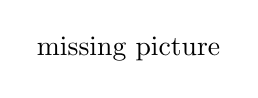
\begin{tikzpicture}
        \node {missing picture};
    \end{tikzpicture}
    \caption{Scalability results for the tandem model}
    \label{fig:tandem_results}
\end{figure}